% !TeX program = xelatex
\documentclass[a4paper,10pt]{article}

% ============================================================================
% កញ្ចប់ស្នូល និងការកំណត់ទំព័រ (តាមគំរូ ls_plan.tex ១០០%)
% ============================================================================
\usepackage[a4paper, left=0.95cm, right=0.95cm, top=0.85cm, bottom=0.92cm, footskip=0.52cm]{geometry}
\usepackage{amsmath}
\usepackage{unicode-math}
\usepackage{fontspec}
\usepackage{longtable, array, colortbl}
\usepackage[table]{xcolor}
\usepackage{enumitem}
\usepackage{pifont}
\usepackage{fancyhdr}
\usepackage{tikz}
\usetikzlibrary{calc, arrows.meta, angles, quotes, patterns, decorations.markings, babel}

% Guard សម្រាប់ការពារកំហុស expl3 លើប្រព័ន្ធ TeX Live ថ្មីៗ
\makeatletter
\let\@expl@@@mark@update@singlecol@structures@@\relax
\makeatother

% ============================================================================
% ការកំណត់ពុម្ពអក្សរ (Cross-Platform Font Resolver: Windows Local + Linux Cloud)
% ============================================================================
\providecommand{\NGSFindFonts}{%
  \IfFileExists{C:/Windows/Fonts/cambria.ttc}{%
    \def\NGSSysPath{C:/Windows/Fonts/}%
    \def\NGSUserPath{C:/Users/KIT/AppData/Local/Microsoft/Windows/Fonts/}%
  }{%
    \IfFileExists{./fonts/KhmerOSsiemreap.ttf}{\def\NGSSysPath{./fonts/}\def\NGSUserPath{./fonts/}}{%
    \IfFileExists{../fonts/KhmerOSsiemreap.ttf}{\def\NGSSysPath{../fonts/}\def\NGSUserPath{../fonts/}}{%
    \IfFileExists{../../fonts/KhmerOSsiemreap.ttf}{\def\NGSSysPath{../../fonts/}\def\NGSUserPath{../../fonts/}}{%
    \IfFileExists{../../../fonts/KhmerOSsiemreap.ttf}{\def\NGSSysPath{../../../fonts/}\def\NGSUserPath{../../../fonts/}}{%
    \IfFileExists{../../../../fonts/KhmerOSsiemreap.ttf}{\def\NGSSysPath{../../../../fonts/}\def\NGSUserPath{../../../../fonts/}}{%
    \IfFileExists{../../../../../fonts/KhmerOSsiemreap.ttf}{\def\NGSSysPath{../../../../../fonts/}\def\NGSUserPath{../../../../../fonts/}}{%
    \IfFileExists{../../../../../../fonts/KhmerOSsiemreap.ttf}{\def\NGSSysPath{../../../../../../fonts/}\def\NGSUserPath{../../../../../../fonts/}}{%
      \def\NGSSysPath{../../../../../../../fonts/}\def\NGSUserPath{../../../../../../../fonts/}%
    }}}}}}}%
  }%
}
\NGSFindFonts

% គណិតវិទ្យាប្រើ Cambria Math ជាមូលដ្ឋាន
\setmathfont[Path={\NGSSysPath}, FontIndex=1, Scale=1.02]{cambria.ttc}
\defaultfontfeatures{Ligatures=TeX}

% អក្សរខ្មែរតួមេ៖ Khmer OS Siemreap
\setmainfont[
  Path={\NGSUserPath},
  Extension=.ttf,
  Script=Khmer,
  BoldFont={KhmerOSsiemreap},
  BoldFeatures={FakeBold=1.8},
  ItalicFont={KhmerOSsiemreap},
  ItalicFeatures={FakeSlant=0.25},
  BoldItalicFont={KhmerOSsiemreap},
  BoldItalicFeatures={FakeBold=1.8, FakeSlant=0.25}
]{KhmerOSsiemreap}

% អក្សរឆ្លាក់ខ្មែរ៖ Khmer OS Muol Light (ហាមដាក់ FakeBold!)
\newfontfamily\muol[
  Path={\NGSUserPath},
  Extension=.ttf,
  Script=Khmer
]{KhmerOSmuollight}

% ក្បាច់រចនាខ្មែរក្រោមបាវចនា៖ Tacteing
\newfontfamily\Tacteing[
  Path={\NGSUserPath},
  Extension=.TTF
]{TACTENG}

% ពុម្ពអក្សរឡាតាំង Times New Roman, Naga Bold, Calibri, Tacteing & Courier
\newfontfamily\TimesEn[
  Path={\NGSSysPath},
  Extension=.ttf,
  Scale=1.00,
  BoldFont={timesbd},
  ItalicFont={timesi},
  BoldItalicFont={timesbi}
]{times}

\newfontfamily\NagaBold[
  Path={\NGSUserPath},
  Extension=.ttf
]{AKbalthom Naga Bold}

\newfontfamily\CalibriFont[
  Path={\NGSSysPath},
  Extension=.ttf
]{calibri}

\newfontfamily\CourierBullet[
  Path={\NGSSysPath},
  Extension=.ttf
]{cour}
\newcommand{\wcirc}{{\CourierBullet\fontsize{9.5pt}{11pt}\selectfont o}}

% ការកាត់ពាក្យខ្មែរដោយស្វ័យប្រវត្តិ
\XeTeXlinebreaklocale "km"
\XeTeXlinebreakskip = 0pt plus 1pt minus 0.1pt

% ============================================================================
% ពណ៌ ប្លង់ទំព័រ និងម៉ាក្រូជំនួយ
% ============================================================================
\definecolor{stepgray}{HTML}{D9D9D9}
\definecolor{headgray}{HTML}{F2F2F2}
\definecolor{boxgray}{HTML}{E6E6E6}
\definecolor{darkred}{HTML}{C00000}
\definecolor{red5e}{HTML}{FF0000}

\pagestyle{fancy}
\fancyhf{}
\renewcommand{\headrulewidth}{0pt}
\fancyfoot[R]{\CalibriFont\fontsize{11pt}{13pt}\selectfont\thepage}

\setlength{\parindent}{0pt}
\setlength{\parskip}{0pt}
\setlength{\tabcolsep}{3.8pt}
\setlength{\LTpre}{2pt}
\setlength{\LTpost}{2pt}

\newcolumntype{L}[1]{>{\raggedright\arraybackslash}p{#1}}
\newcolumntype{C}[1]{>{\centering\arraybackslash}p{#1}}

\newcommand{\en}[1]{{\TimesEn #1}}
\newcommand{\enbf}[1]{{\TimesEn\textbf{#1}}}
\newcommand{\unit}[1]{\,\text{\en{#1}}}
\newcommand{\fiveE}[1]{{\NagaBold\fontsize{9.5pt}{13pt}\selectfont\textcolor{red5e}{#1}}}
\newcommand{\timenote}[1]{\textcolor{darkred}{\textit{#1}}}
\newcommand{\khmflourish}{{\Tacteing\fontsize{17pt}{17pt}\selectfont 3}}
\newcommand{\graybox}[1]{\colorbox{boxgray}{\strut\hspace{2pt}#1\hspace{2pt}}}
\newcommand{\ditem}{\tikz[baseline=-0.5ex]\fill (0,0.42ex) -- (0.42ex,0) -- (0,-0.42ex) -- (-0.42ex,0) -- cycle;\hspace{0.3em}}
\newcommand{\cnum}[1]{{\fontsize{10.5pt}{12pt}\selectfont\ding{\numexpr181+#1\relax}}\hspace{0.2em}}
\newcommand{\cfig}[1]{\par\vspace{4pt}{\centering #1\par}\vspace{4pt}}
\newcommand{\stepheader}[1]{\multicolumn{3}{|c|}{\cellcolor{stepgray}\muol #1} \\* \noalign{\hrule height 0.4pt}}
\newcommand{\tri}[1]{\ensuremath{\triangle #1}}
\newcommand{\ang}[1]{\ensuremath{\angle #1}}
\newcommand{\chkbox}{\tikz[baseline=-0.15ex]\draw[black, line width=0.8pt] (0,0) rectangle (0.23cm,0.23cm);}

\newcommand{\rightbox}[4][0.18]{%
  \draw[black, line width=0.75pt]
    ($(#3)!#1!(#2)$) -- ($($(#3)!#1!(#2)$)+($(#3)!#1!(#4)$)-(#3)$) -- ($(#3)!#1!(#4)$);
}

% ============================================================================
% រូបធរណីមាត្រ ស-ខ្មៅ (B&W Print-Safe TikZ Figures for 3D Prisms & 2D Nets)
% ============================================================================

% ១. កំណែកិច្ចការផ្ទះទី១១ (ទំ.២១៤) និងរំលឹករូបមន្តផ្ទៃក្រឡារូបវិមាត្រពីរ (មេរៀនទី១៥)
\newcommand{\figPrereqPrism}{%
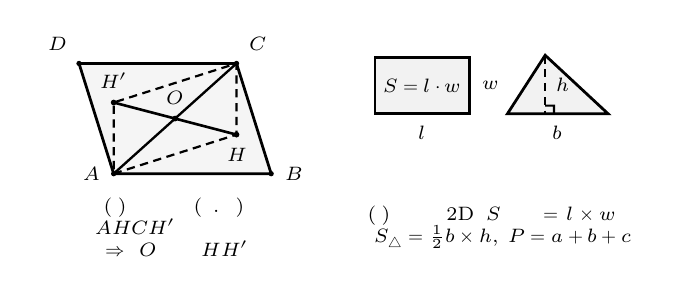
\begin{tikzpicture}[scale=0.80, every node/.style={font=\scriptsize, text=black}]
  % (ក) កំណែលំហាត់ទី១១ ទំ.២១៤៖ ប្រលេឡូក្រាម AHCH' => O កណ្ដាល HH'
  \begin{scope}[shift={(0,0)}]
    \coordinate (A) at (-1.15,-0.80);
    \coordinate (B) at (1.35,-0.80);
    \coordinate (C) at (0.80,0.95);
    \coordinate (D) at (-1.70,0.95);
    \coordinate (O) at (-0.175,0.075);
    \coordinate (H) at (0.80,-0.18);
    \coordinate (Hp) at (-1.15,0.33);
    \fill[gray!8] (A) -- (B) -- (C) -- (D) -- cycle;
    \draw[black, line width=1.0pt] (A) -- (B) -- (C) -- (D) -- cycle;
    \draw[black, line width=0.85pt] (A) -- (C);
    \draw[black, line width=0.95pt] (H) -- (Hp);
    \draw[black, line width=0.8pt, densely dashed] (A) -- (H) -- (C) -- (Hp) -- (A);
    \fill[black] (A) circle (1.2pt) node[left=1.5pt] {$A$};
    \fill[black] (B) circle (1.2pt) node[right=1.5pt] {$B$};
    \fill[black] (C) circle (1.2pt) node[above right=1pt] {$C$};
    \fill[black] (D) circle (1.2pt) node[above left=1pt] {$D$};
    \fill[black] (O) circle (1.3pt) node[above=1.5pt] {$O$};
    \fill[black] (H) circle (1.3pt) node[below=1.5pt] {$H$};
    \fill[black] (Hp) circle (1.3pt) node[above=1.5pt] {$H'$};
    \node[align=center, text width=3.55cm] at (-0.15,-1.65) {(ក) លំហាត់ទី១១ (ទំ.២១៤)៖\\$AHCH'$ ជាប្រលេឡូក្រាម $\Rightarrow O$ កណ្ដាល $HH'$};
  \end{scope}

  % (ខ) រំលឹកផ្ទៃក្រឡារូប 2D៖ ចតុកោណកែង និងត្រីកោណ
  \begin{scope}[shift={(4.55,0)}]
    \draw[black, line width=1.0pt, fill=gray!10] (-1.55,0.15) rectangle (-0.05,1.05);
    \node at (-0.80,0.60) {$S=l\cdot w$};
    \node[below=1pt] at (-0.80,0.15) {$l$};
    \node[right=1pt] at (-0.05,0.60) {$w$};

    \coordinate (T1) at (0.55,0.15);
    \coordinate (T2) at (2.15,0.15);
    \coordinate (T3) at (1.15,1.08);
    \coordinate (TF) at (1.15,0.15);
    \draw[black, line width=1.0pt, fill=gray!10] (T1) -- (T2) -- (T3) -- cycle;
    \draw[black, line width=0.8pt, densely dashed] (T3) -- (TF) node[midway, right=0.5pt] {$h$};
    \rightbox[0.14]{T3}{TF}{T2}
    \node[below=1pt] at (1.35,0.15) {$b$};
    \node[align=center, text width=3.65cm] at (0.30,-1.65) {(ខ) រំលឹករូប 2D៖ $S_{\text{ចតុកោណកែង}}=l\times w$\\និង $S_{\tri{}}=\frac{1}{2}b\times h,\; P=a+b+c$};
  \end{scope}
\end{tikzpicture}}

% ២. E1 Engage: តង់កៅស៊ូរាងព្រីសត្រង់ត្រីមុខដេក (លំហាត់គំរូទី 1 ទំ.២១៧៖ តើមុខណាជាបាតព្រីស?)
\newcommand{\figEngagePrism}{%
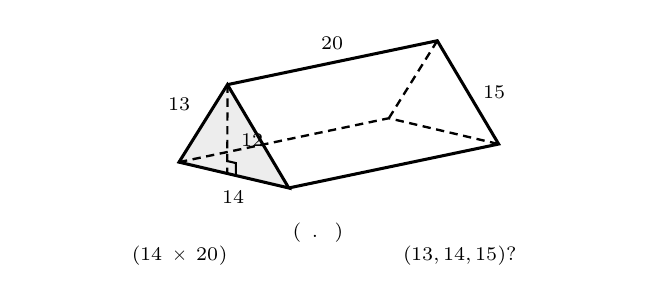
\begin{tikzpicture}[scale=0.82, every node/.style={font=\scriptsize, text=black}]
  \coordinate (A) at (-2.40,-0.45);
  \coordinate (B) at (-0.70,-0.85);
  \coordinate (C) at (-1.65,0.75);
  \coordinate (Shift) at (3.25,0.68);
  \coordinate (Ap) at ($(A)+(Shift)$);
  \coordinate (Bp) at ($(B)+(Shift)$);
  \coordinate (Cp) at ($(C)+(Shift)$);
  \coordinate (H) at ($(A)!0.44!(B)$);

  \fill[gray!14] (A) -- (B) -- (C) -- cycle;
  \draw[black, line width=1.1pt] (A) -- (B) -- (C) -- cycle;
  \draw[black, line width=1.1pt] (B) -- (Bp) -- (Cp) -- (C);
  \draw[black, line width=0.85pt, densely dashed] (A) -- (Ap) -- (Bp) (Ap) -- (Cp);
  \draw[black, line width=0.8pt, densely dashed] (C) -- (H);
  \node[right=1.5pt] at ($0.38*(C)+0.62*(H)$) {$12$};
  \rightbox[0.14]{C}{H}{B}

  \node[above left=1pt] at ($0.5*(A)+0.5*(C)$) {$13$};
  \node[below=2pt] at ($0.5*(A)+0.5*(B)$) {$14$};
  \node[above=1pt] at ($0.5*(C)+0.5*(Cp)$) {$20$};
  \node[right=2pt] at ($0.5*(Bp)+0.5*(Cp)$) {$15$};

  \node[align=center, text width=7.3cm] at (-0.15,-1.72) {តង់រាងព្រីសត្រង់ត្រីមុខដេក (ទំ.២១៧)៖ តើ \textbf{បាតព្រីស} គឺមុខក្រោមបាតដី ($14\times 20$) ឬមុខត្រីកោណពីរស្របគ្នាប៉ុនគ្នា ($13,14,15$)?};
\end{tikzpicture}}

% ៣. E2/E3 ការលាតប្លង់ 2D នៃព្រីសត្រង់ត្រីមុខ (លំហាត់គំរូទី 1 ទំ.២១៧៖ Sl = P*h = 840, St = Sl + 2B = 1008)
\newcommand{\figPrismNetProof}{%
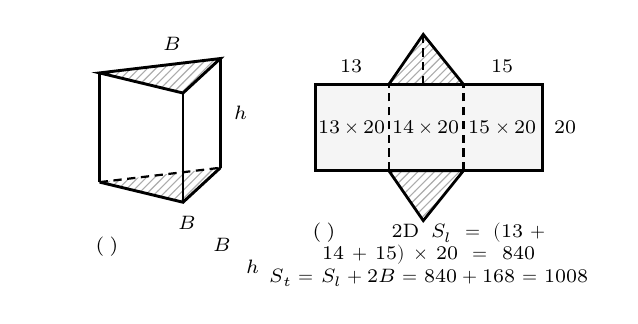
\begin{tikzpicture}[scale=0.73, every node/.style={font=\scriptsize, text=black}]
  % ខាងឆ្វេង៖ ធាតុនៃព្រីសត្រង់ (បាត ២ ស្របគ្នាប៉ុនគ្នា + ទ្រនុងខាង h + មុខខាង)
  \begin{scope}[shift={(-2.55,0.10)}]
    \coordinate (A1) at (-1.15,-0.95);
    \coordinate (B1) at (0.30,-1.30);
    \coordinate (C1) at (0.95,-0.70);
    \coordinate (A2) at (-1.15,0.95);
    \coordinate (B2) at (0.30,0.60);
    \coordinate (C2) at (0.95,1.20);
    \fill[pattern=north east lines, pattern color=gray!65] (A1) -- (B1) -- (C1) -- cycle;
    \fill[pattern=north east lines, pattern color=gray!65] (A2) -- (B2) -- (C2) -- cycle;
    \draw[black, line width=1.05pt] (A2) -- (B2) -- (C2) -- cycle;
    \draw[black, line width=1.05pt] (A1) -- (B1) -- (C1);
    \draw[black, line width=0.8pt, densely dashed] (A1) -- (C1);
    \draw[black, line width=1.05pt] (A1) -- (A2) (B1) -- (B2) (C1) -- (C2);
    \node[right=1.5pt] at ($0.5*(C1)+0.5*(C2)$) {$h$};
    \node[above=2pt] at (-0.10,1.08) {\textbf{បាត $B$}};
    \node[below=2pt] at (0.15,-1.28) {\textbf{បាត $B$}};
    \node[align=center, text width=3.2cm] at (-0.05,-2.22) {(ក) ព្រីសត្រង់៖ បាត $B$ ពីរស្របគ្នាប៉ុនគ្នា និងទ្រនុងខាង $h$};
  \end{scope}

  % ខាងស្ដាំ៖ គំនូសលាត 2D នៃលំហាត់គំរូទី 1 (P = 13+14+15 = 42, h = 20)
  \begin{scope}[shift={(1.95,0.10)}]
    \draw[black, line width=1.05pt, fill=gray!8] (-1.90,-0.75) rectangle (2.05,0.75);
    \draw[black, line width=0.85pt, densely dashed] (-0.62,-0.75) -- (-0.62,0.75);
    \draw[black, line width=0.85pt, densely dashed] (0.68,-0.75) -- (0.68,0.75);
    % បាតត្រីកោណពីរ (ឆ្នូតបញ្ឆិត)
    \fill[pattern=north east lines, pattern color=gray!65] (-0.62,0.75) -- (0.68,0.75) -- (-0.02,1.62) -- cycle;
    \draw[black, line width=1.0pt] (-0.62,0.75) -- (0.68,0.75) -- (-0.02,1.62) -- cycle;
    \draw[black, line width=0.75pt, densely dashed] (-0.02,1.62) -- (-0.02,0.75);
    \fill[pattern=north east lines, pattern color=gray!65] (-0.62,-0.75) -- (0.68,-0.75) -- (-0.02,-1.62) -- cycle;
    \draw[black, line width=1.0pt] (-0.62,-0.75) -- (0.68,-0.75) -- (-0.02,-1.62) -- cycle;

    \node at (-1.26,0) {$13\times 20$};
    \node at (0.03,0) {$14\times 20$};
    \node at (1.36,0) {$15\times 20$};
    \node[right=1pt] at (2.05,0) {$20$};
    \node[above=0.5pt] at (-1.26,0.75) {$13$};
    \node[above=0.5pt] at (1.36,0.75) {$15$};
    \node[align=center, text width=4.35cm] at (0.08,-2.22) {(ខ) គំនូសលាត \en{2D}៖ $S_l = (13+14+15)\times 20 = 840$\\$S_t = S_l + 2B = 840 + 168 = 1008$};
  \end{scope}
\end{tikzpicture}}

% ៤. E4 លំហាត់គំរូទី 2 និងប្រតិបត្តិ រូប ក, រូប ខ (ទំ.២១៧)
\newcommand{\figElaboratePrism}{%
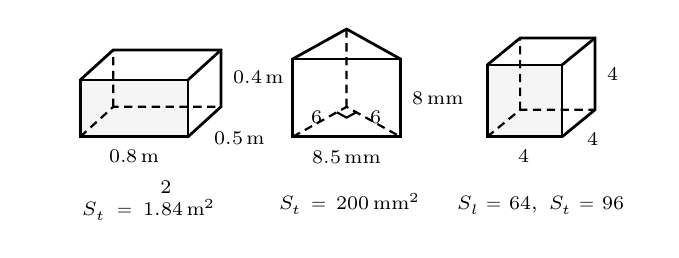
\begin{tikzpicture}[scale=0.76, every node/.style={font=\scriptsize, text=black}]
  % (១) លំហាត់គំរូទី 2៖ 0.8m x 0.5m x 0.4m
  \begin{scope}[shift={(-3.15,0)}]
    \draw[black, line width=1.0pt, fill=gray!8] (-1.10,-0.65) rectangle (0.70,0.30);
    \draw[black, line width=1.0pt] (0.70,-0.65) -- (1.25,-0.15) -- (1.25,0.80) -- (-0.55,0.80) -- (-1.10,0.30);
    \draw[black, line width=1.0pt] (0.70,0.30) -- (1.25,0.80);
    \draw[black, line width=0.8pt, densely dashed] (-1.10,-0.65) -- (-0.55,-0.15) -- (1.25,-0.15) (-0.55,-0.15) -- (-0.55,0.80);
    \node[below=1pt] at (-0.20,-0.65) {$0.8\unit{m}$};
    \node[below right=0pt] at (0.98,-0.40) {$0.5\unit{m}$};
    \node[right=1pt] at (1.25,0.35) {$0.4\unit{m}$};
    \node[align=center, text width=2.85cm] at (0.05,-1.72) {គំរូទី \en{2}៖\\$S_t=1.84\unit{m}^2$};
  \end{scope}

  % (២) ប្រតិបត្តិ រូប ក៖ 6mm, 6mm, 8.5mm, h=8mm
  \begin{scope}[shift={(0.25,0)}]
    \coordinate (L1) at (-0.95,-0.65);
    \coordinate (R1) at (0.85,-0.65);
    \coordinate (M1) at (-0.05,-0.15);
    \coordinate (L2) at (-0.95,0.65);
    \coordinate (R2) at (0.85,0.65);
    \coordinate (M2) at (-0.05,1.15);
    \draw[black, line width=1.0pt] (L1) -- (R1) -- (R2) -- (L2) -- cycle;
    \draw[black, line width=1.0pt] (L2) -- (M2) -- (R2);
    \draw[black, line width=0.8pt, densely dashed] (L1) -- (M1) -- (R1) (M1) -- (M2);
    \rightbox[0.18]{L1}{M1}{R1}
    \node[below=1.5pt] at (-0.05,-0.65) {$8.5\unit{mm}$};
    \node[right=1pt] at (0.85,0) {$8\unit{mm}$};
    \node at (-0.55,-0.32) {$6$};
    \node at (0.45,-0.32) {$6$};
    \node[align=center, text width=2.65cm] at (0.0,-1.72) {ប្រតិបត្តិ រូប ក៖\\$S_t=200\unit{mm}^2$};
  \end{scope}

  % (៣) ប្រតិបត្តិ រូប ខ៖ គូបជ្រុង 4
  \begin{scope}[shift={(3.35,0)}]
    \draw[black, line width=1.0pt, fill=gray!8] (-0.80,-0.65) rectangle (0.45,0.55);
    \draw[black, line width=1.0pt] (0.45,-0.65) -- (1.00,-0.20) -- (1.00,1.00) -- (-0.25,1.00) -- (-0.80,0.55);
    \draw[black, line width=1.0pt] (0.45,0.55) -- (1.00,1.00);
    \draw[black, line width=0.8pt, densely dashed] (-0.80,-0.65) -- (-0.25,-0.20) -- (1.00,-0.20) (-0.25,-0.20) -- (-0.25,1.00);
    \node[below=1pt] at (-0.18,-0.65) {$4$};
    \node[below right=0pt] at (0.72,-0.42) {$4$};
    \node[right=1pt] at (1.00,0.40) {$4$};
    \node[align=center, text width=2.55cm] at (0.10,-1.72) {ប្រតិបត្តិ រូប ខ៖\\$S_l=64,\; S_t=96$};
  \end{scope}
\end{tikzpicture}}

% ============================================================================
% ចាប់ផ្ដើមឯកសារ (Document Body)
% ============================================================================
\begin{document}
\fontsize{10pt}{15.2pt}\selectfont

% -------------------- ក្បាលកិច្ចតែងការ (Header) --------------------
\begin{center}
  {\muol\fontsize{11pt}{16pt}\selectfont ព្រះរាជាណាចក្រកម្ពុជា}\\[2pt]
  {\muol\fontsize{10pt}{15pt}\selectfont ជាតិ សាសនា ព្រះមហាក្សត្រ}\\[1pt]
  \khmflourish
\end{center}

\vspace{-26pt}
{\muol\fontsize{9.5pt}{12.8pt}\selectfont
មន្ទីរអប់រំ យុវជន និងកីឡា ខេត្តកំពង់ធំ\\
ការិយាល័យអប់រំ យុវជន និងកីឡា ស្រុកកំពង់ស្វាយ\\
អនុវិទ្យាល័យព្រះក្រសាំង}

\vspace{1pt}
\begin{center}
  {\muol\fontsize{10pt}{14.5pt}\selectfont កិច្ចតែងការបង្រៀន}
\end{center}
\vspace{0pt}

% -------------------- ព័ត៌មានទូទៅ (Metadata) --------------------
{\renewcommand{\arraystretch}{0.98}
\hspace*{4.05cm}%
\begin{tabular}{@{}l l l@{}}
  - \hspace{0.35cm} មុខវិជ្ជា & : & គណិតវិទ្យា ថ្នាក់ទី៨ \\
  - \hspace{0.35cm} ចំណងជើងមេរៀន & : & មេរៀនទី១៧ រូបធរណីមាត្រដែលមានវិមាត្របី \\
  - \hspace{0.35cm} ចំណងជើងរង & : & ១៧.១ សញ្ញាណសូលីត និងផ្ទៃក្រឡានៃព្រីស (ទំព័រ ២១៥--២១៧) \\
  - \hspace{0.35cm} រយៈពេល & : & ១ ម៉ោងសិក្សា (៥០ នាទី) \\
  - \hspace{0.35cm} បង្រៀនដោយ & : & ហុក ប៊ុនថែន \\
  - \hspace{0.35cm} កាលបរិច្ឆេទ & : & ថ្ងៃ\makebox[18mm]{\dotfill}\ ទី\makebox[8mm]{\dotfill}\ ខែ\makebox[18mm]{\dotfill}\ ឆ្នាំ២០២៦ \\
\end{tabular}

\vspace{2pt}

% -------------------- I. វត្ថុបំណង --------------------
\textbf{I.} {\muol វត្ថុបំណង}\\[1pt]
\hspace*{0.55cm}%
\begin{tabular}{@{}l l L{14.2cm}@{}}
  \wcirc \hspace{0.25cm} វិជ្ជាសម្បទា & : & សិស្សប្រាប់បានត្រឹមត្រូវពីសញ្ញាណសូលីត ពហុមុខ ធាតុនៃព្រីស (បាតពីរស្របគ្នាប៉ុនគ្នា ទ្រនុងខាង មុខខាង ព្រីសត្រង់ទល់នឹងព្រីសទ្រេត) និងរូបមន្តផ្ទៃក្រឡាខាង ($S_l$) ព្រមទាំងផ្ទៃក្រឡាទាំងអស់ ($S_t=S_l+2B$) នៃព្រីសត្រង់ ។ \\
  \wcirc \hspace{0.25cm} បំណិនសម្បទា & : & សិស្សកំណត់បាតព្រីសបានត្រឹមត្រូវទោះបីព្រីសស្ថិតក្នុងទម្រង់ដេក ភ្ជាប់រូបព្រីស \en{3D} ទៅគំនូសលាត \en{2D} លើសន្លឹកកិច្ចការ និងគណនាផ្ទៃក្រឡាខាងនិងផ្ទៃក្រឡាទាំងអស់នៃព្រីសត្រង់បានត្រឹមត្រូវ ។ \\
  \wcirc \hspace{0.25cm} ចរិយាសម្បទា & : & សិស្សមានទម្លាប់ពិនិត្យវិភាគមុខទាំងអស់នៃរូបធរណីមាត្រវិមាត្របីដោយហ្មត់ចត់ (មិនច្រឡំមុខក្រោមជាបាតព្រីស) និងសហការគ្នាដោះស្រាយបញ្ហាជាក់ស្ដែងយ៉ាងសកម្ម ។ \\
\end{tabular}

\vspace{2pt}

% -------------------- II. សម្ភារៈឧបទេស --------------------
\textbf{II.} {\muol សម្ភារៈឧបទេស}\\[1pt]
\hspace*{0.55cm}$\bullet$ \hspace{0.35cm} សៀវភៅសិក្សាគោលគណិតវិទ្យាថ្នាក់ទី៨ (ទំ.២១៥--២១៧ និង ២២៦--២២៧) សន្លឹកកិច្ចការសិស្ស ស-ខ្មៅ (\en{Worksheet\_PRISM\_SA} ចំនួន ២ ទំព័រ គ្មាន \en{LCD}) ប្រអប់ដីសលើតុគ្រូ ក្ដារខៀន ដីស និងបន្ទាត់ក្រិត ។

\vspace{2pt}

% -------------------- III. វិធីសាស្រ្តបង្រៀន --------------------
\textbf{III.} {\muol វិធីសាស្រ្តបង្រៀន}\\[1pt]
\hspace*{0.45cm}%
\begin{tabular}{@{}l l L{14.85cm}@{}}
  $\bullet$ \hspace{0.25cm} គោលវិធី & : & សិស្សមជ្ឈមណ្ឌល (សិក្សាតាមរយៈការវិភាគគំនូសលាត \en{2D} និងបំពេញលើសន្លឹកកិច្ចការជាគោល គ្មាន \en{LCD}) \\
  $\bullet$ \hspace{0.25cm} យុទ្ធវិធីបង្រៀន & : & ស្ថាបនានិយម គម្រូ \en{5Es} រួមបញ្ចូលឧទាហរណ៍ទល់នឹងមិនមែនឧទាហរណ៍ (\en{Examples \& Non-Examples}), ការលាតប្លង់សូលីត (\en{3D-to-2D Net Unfolding}) និងការវិនិច្ឆ័យកំហុស (\en{Spot-the-Error}) ។ \\
\end{tabular}
}

\vspace{2pt}

% -------------------- IV. ដំណើរការបង្រៀន --------------------
\textbf{IV.} {\muol ដំណើរការបង្រៀន}

\vspace{1pt}

\renewcommand{\arraystretch}{1.15}
\begin{longtable}{|L{5.50cm}|L{7.90cm}|L{4.80cm}|}
\hline
\rowcolor{headgray}
\multicolumn{1}{|c|}{\muol សកម្មភាពគ្រូ} &
\multicolumn{1}{c|}{\muol ខ្លឹមសារមេរៀន} &
\multicolumn{1}{c|}{\muol សកម្មភាពសិស្ស} \\
\hline
\endfirsthead

\hline
\rowcolor{headgray}
\multicolumn{1}{|c|}{\muol សកម្មភាពគ្រូ} &
\multicolumn{1}{c|}{\muol ខ្លឹមសារមេរៀន} &
\multicolumn{1}{c|}{\muol សកម្មភាពសិស្ស} \\
\hline
\endhead

\hline
\endfoot

\hline
\endlastfoot

% ==================== ជំហានទី១ (2 min) ====================
\stepheader{ជំហានទី១ (រដ្ឋបាលថ្នាក់)}
$\bullet$ ពិនិត្យវត្តមាន សណ្ដាប់ធ្នាប់ អនាម័យ និងចែកសន្លឹកកិច្ចការ \en{Worksheet\_PRISM\_SA} ដល់សិស្សគ្រប់គូ \timenote{(2 min)}
&
$\bullet$ រដ្ឋបាលថ្នាក់ និងការត្រៀមសៀវភៅគោល បន្ទាត់ក្រិត និងសន្លឹកកិច្ចការសិស្ស
&
$\circ$ ប្រធានថ្នាក់រាយការណ៍វត្តមាន\par\vspace{2pt}
$\circ$ ទទួលសន្លឹកកិច្ចការ និងត្រៀមឧបករណ៍ \\[3pt]
\hline

% ==================== ជំហានទី២ (9 min: ≤3 + 3 + E1 3) ====================
\stepheader{ជំហានទី២ (កិច្ចការផ្ទះ + រំលឹកមេរៀនចាស់ + ទំនាក់ទំនងមេរៀនថ្មី)}
\timenote{(កំណែកិច្ចការផ្ទះ $\le 3\text{ min}$)}\par\vspace{1.5pt}
$\bullet$ ហៅសិស្សបង្ហាញកំណែលំហាត់ទី១១ (ទំ.២១៤) យ៉ាងរហ័សលើក្ដារខៀន
&
\textbf{កំណែកិច្ចការផ្ទះ (ទំ.២១៤ លំហាត់ទី១១)៖}\par\vspace{1.5pt}
$\bullet$ ដោយ $BC\parallel AD$: $AH\perp BC \Rightarrow AH\perp AD$ និង $CH'\perp AD \Rightarrow AH\parallel CH'$ ។ ដូចគ្នា $CH\perp AB,\; AH'\perp CD \Rightarrow CH\parallel AH'$ ។\par\vspace{1.5pt}
$\bullet$ ដូចនេះ $AHCH'$ ជាប្រលេឡូក្រាម ដែលអង្កត់ទ្រូង $AC$ និង $HH'$ កាត់គ្នាត្រង់ចំណុចកណ្ដាល $O \Rightarrow$ \graybox{$O$ ជាចំណុចកណ្ដាលនៃ $HH'$} ។
&
$\circ$ តំណាងឡើងសរសេរគន្លឹះកំណែ\par\vspace{2pt}
$\circ$ ផ្ទៀងផ្ទាត់និងកែក្នុងសៀវភៅសរសេរ \\[3pt]

\timenote{(រំលឹកមេរៀនចាស់ 3 min)}\par\vspace{1pt}
$\bullet$ សួរ៖ «តើផ្ទៃក្រឡាចតុកោណកែង និងការេគណនាតាមរូបមន្តអ្វី?»
&
\textbf{រំលឹកបញ្ញត្តិមេរៀនទី១៥ (រូបធរណីមាត្រវិមាត្រពីរ)៖}\par\vspace{1pt}
\ditem ចតុកោណកែង៖ $S = l \times w$ \;\textbar\; ការេ៖ $S = a^2$ ។
&
$\circ$ ឆ្លើយរំលឹករូបមន្តផ្ទៃក្រឡាចតុកោណកែង និងការេ \\[3pt]

$\bullet$ សួរបន្ត៖ «ចុះផ្ទៃក្រឡានិងបរិមាត្រត្រីកោណដែលមានជ្រុង $a,b,c$ គណនាដូចម្ដេច?»
&
\ditem ត្រីកោណ៖ $S = \dfrac{1}{2}b \times h$ និងបរិមាត្រ $P = a + b + c$ ។
&
$\circ$ ឆ្លើយរំលឹករូបមន្តផ្ទៃក្រឡានិងបរិមាត្រត្រីកោណ \\[3pt]

& \cfig{\figPrereqPrism} & \\[3pt]

\fiveE{E1 - Engage} \timenote{(3 min)}\par\vspace{1.5pt}
$\bullet$ លើកប្រអប់ដីសបង្ហាញធៀបនឹងរូបតង់លើ \textbf{បេសកកម្មទី១ (\en{E1})} នៃសន្លឹកកិច្ចការ៖\par\vspace{1pt}
\hspace*{0.3em}-- «តង់កៅស៊ូរាងព្រីសត្រង់ត្រីមុខដាក់ដេកលើដីតាមមុខចតុកោណកែង $14\times 20$ ហើយមុខត្រីកោណមុខ-ក្រោយមានជ្រុង $13,14,15$ (កម្ពស់ $12$) ។ សិស្ស ក ថា បាតព្រីសគឺមុខក្រោមបាតដី $14\times 20$ ឯសិស្ស ខ ថា បាតព្រីសគឺមុខត្រីកោណទាំងពីរ! តើអ្នកណាត្រឹមត្រូវ?»
&
\textbf{មេរៀនទី១៧៖ រូបធរណីមាត្រដែលមានវិមាត្របី}\par\vspace{1.5pt}
\textbf{១៧.១ ផ្ទៃក្រឡាខាង និងផ្ទៃក្រឡាទាំងអស់នៃព្រីស}\par\vspace{1.5pt}
\ditem \textbf{បញ្ហាបំផុសគំនិត (\en{E1})៖} ការកំណត់ «បាតព្រីស» ឱ្យត្រឹមត្រូវពេលព្រីសត្រីមុខស្ថិតក្នុងទម្រង់ដេក និងការគណនាផ្ទៃក្រឡាកៅស៊ូធ្វើតង់ទាំងមូល ។
&
$\circ$ សង្កេតប្រអប់ដីសនិងរូបតង់លើសន្លឹកកិច្ចការ\par\vspace{2pt}
$\circ$ គូសធីកទស្សន៍ទាយជាដៃគូ \\[3pt]

& \cfig{\figEngagePrism} & \\[3pt]
\hline

% ==================== ជំហានទី៣ (17 min: E2 11 + E3 6) ====================
\stepheader{ជំហានទី៣ (ខ្លឹមសារមេរៀនថ្មី)}
\fiveE{E2 - Explore} \timenote{(11 min: 5 min)}\par\vspace{1pt}
$\bullet$ ឱ្យសិស្សធ្វើជាដៃគូលើ \textbf{ផ្នែកទី១ (ក) ស្គាល់សូលីត ពហុមុខ និងបាតព្រីស} (ទំ.២១៥--២១៦)
&
\textbf{សកម្មភាពរុករកទី១ (ឧទាហរណ៍ និងមិនមែនឧទាហរណ៍នៃព្រីស)៖}\par\vspace{1pt}
$1.$ សូលីតមានវិមាត្របី (បណ្តោយ ទទឹង កម្ពស់); សូលីតមានមុខច្រើនហៅថា \textbf{ពហុមុខ} ។
&
$\circ$ ពិនិត្យរូបសូលីតទាំង ៤ លើសន្លឹកកិច្ចការ \\[3pt]

$\bullet$ ដើរសួរ៖ «ហេតុអ្វីរូបទី២ (ព្រីសត្រីមុខដេក) មានបាតជាត្រីកោណ មិនមែនចតុកោណកែងក្រោម? ចុះរូបទី៤ (ពីរ៉ាមីត) ជាព្រីសឬទេ?»
&
$2.$ ក្នុងព្រីសត្រីមុខដេក មានតែមុខ \textbf{ត្រីកោណទាំងពីរ} ប៉ុណ្ណោះដែលស្របគ្នានិងប៉ុនគ្នា (ជា \textbf{បាតព្រីស}); ឯពីរ៉ាមីតមានបាតតែមួយ (មិនមែនព្រីសទេ)!
&
$\circ$ គូសឆ្នូតបញ្ឆិតលើបាតពីរស្របគ្នាប៉ុនគ្នា និងបែងចែកព្រីសពីពីរ៉ាមីត \\[3pt]

\timenote{(E2 ទី២៖ គំនូសលាត \en{2D} លំហាត់គំរូទី \en{1} — 6 min)}\par\vspace{1.5pt}
$\bullet$ ដឹកនាំសិស្សបំពេញ \textbf{ផ្នែកទី១ (ខ) គំនូសលាត \en{2D} នៃព្រីសត្រង់ត្រីមុខ} (លំហាត់គំរូទី \en{1} ទំ.២១៧)៖ «ពេលលាតមុខខាងទាំង ៣ តើបានរូបអ្វី?»\par\vspace{24pt}\null
&
\textbf{សកម្មភាពរុករកទី២ — លំហាត់គំរូទី \en{1} (ទំ.២១៧)៖}\par\vspace{1.5pt}
$\bullet$ មុខខាងទាំង ៣ ជាចតុកោណកែង៖\par\vspace{1pt}
\hspace*{0.2em}$S_l = 13\times 20 + 14\times 20 + 15\times 20 = 260+280+300 = \mathbf{840}$ ឯកតាផ្ទៃ\par\vspace{1pt}
\hspace*{0.2em}(ឬចតុកោណកែងលាតធំ៖ $S_l = P\times h = (13+14+15)\times 20 = 840$) ។\par\vspace{24pt}\null
&
$\circ$ ភ្ជាប់ជ្រុង $13,14,15$ ទៅគំនូសលាត \en{2D} និងគណនា $S_l=840$ \\[3pt]

$\bullet$ សួរបន្ត៖ «បើបូកថែមផ្ទៃបាតត្រីកោណទាំងពីរ ($b=14, h_{\text{បាត}}=12$) តើផ្ទៃក្រឡាទាំងអស់ $S_t$ ស្មើប៉ុន្មាន?»
&
$\bullet$ ផ្ទៃបាតមួយ $B = \dfrac{12\times 14}{2} = 84 \Rightarrow 2B = 168$ ឯកតាផ្ទៃ ។\par\vspace{1pt}
$\bullet$ ផ្ទៃក្រឡាទាំងអស់៖ $S_t = S_l + 2B = 840 + 168 = \graybox{$1008\text{ ឯកតាផ្ទៃ}$}$ ។
&
$\circ$ គណនាផ្ទៃបាតទាំងពីរ $2B=168$ និង $S_t = 1008$ ឯកតាផ្ទៃ \\[3pt]

& \cfig{\figPrismNetProof} & \\[3pt]

\fiveE{E3 - Explain} \timenote{(6 min)}\par\vspace{1.5pt}
$\bullet$ ហៅតំណាងគូបង្ហាញ រួចគ្រូសង្ខេបនិយមន័យធាតុនៃព្រីស (ទំ.២១៦) លើក្ដារខៀន ឱ្យសិស្សបំពេញ \textbf{ផ្នែកទី២}
&
\textbf{និយមន័យ និងធាតុនៃព្រីស (ទំ.២១៦)៖}\par\vspace{1.5pt}
$\bullet$ \textbf{បាតព្រីស ($B$)៖} មុខពីរស្របគ្នា ហើយប៉ុនគ្នា (ហៅឈ្មោះព្រីសតាមពហុកោណបាត៖ ព្រីសត្រីមុខ ព្រីសចតុមុខ ព្រីសបញ្ចមុខ) ។\par\vspace{1pt}
$\bullet$ \textbf{ទ្រនុងខាង៖} ជ្រុងស្របគ្នាភ្ជាប់កំពូលទាំងពីរនៃបាត ។ \textbf{មុខខាង៖} មុខមិនមែនជាបាត (ជាប្រលេឡូក្រាម; បើ \textbf{ព្រីសត្រង់} ទ្រនុងខាងកែងនឹងបាត មុខខាងជាចតុកោណកែង) ។
&
$\circ$ តំណាងគូឡើងបកស្រាយ\par\vspace{2pt}
$\circ$ បំពេញនិយមន័យធាតុនៃព្រីសលើសន្លឹកកិច្ចការ \\[3pt]

$\bullet$ សង្ខេបរូបមន្តផ្ទៃក្រឡាខាង $S_l$ និងផ្ទៃក្រឡាទាំងអស់ $S_t$ ព្រមទាំងធនាគារហេតុផល \cnum{1}--\cnum{4}
&
\textbf{រូបមន្តផ្ទៃក្រឡានៃព្រីសត្រង់ (ទំ.២១៦)៖}\par\vspace{1.5pt}
$\bullet$ ផ្ទៃក្រឡាខាង៖ \graybox{$S_l = P \times h$} (ផលបូកផ្ទៃមុខខាងទាំងអស់; $P$ បរិមាត្របាត, $h$ កម្ពស់/ទ្រនុងខាងព្រីស) ។\par\vspace{1.5pt}
$\bullet$ ផ្ទៃក្រឡាទាំងអស់៖ \graybox{$S_t = S_l + 2B$} ($B$ ផ្ទៃក្រឡាបាតមួយ) ។\par\vspace{1.5pt}
$\bullet$ \textbf{ធនាគារហេតុផល៖} \cnum{1} បាតពីរស្របគ្នាប៉ុនគ្នា \;\textbar\; \cnum{2} $S_l = P\times h$ \;\textbar\; \cnum{3} $S_t = S_l + 2B$ \;\textbar\; \cnum{4} $B_{\tri{}}=\frac{1}{2}bh,\; B_{\text{ចតុកោណកែង}}=lw$
&
$\circ$ បំពេញប្រអប់រូបមន្ត $S_l, S_t$ និងផ្ទៀងផ្ទាត់ធនាគារហេតុផល \cnum{1}--\cnum{4} \\[3pt]
\hline

% ==================== ជំហានទី៤ (20 min: E4 10 + E5 10) ====================
\stepheader{ជំហានទី៤ (ពង្រីកចំណេះដឹង និងវាយតម្លៃ)}
\fiveE{E4 - Elaborate} \timenote{(10 min: 5 min)}\par\vspace{1pt}
$\bullet$ ដឹកនាំសិស្សដោះស្រាយ \textbf{ផ្នែកទី៣ (ក) លំហាត់គំរូទី \en{2} (ទំ.២១៧)} លើសន្លឹកកិច្ចការទំព័រទី២៖ ព្រីសត្រង់ចតុមុខ ($0.8\unit{m},\; 0.5\unit{m},\; 0.4\unit{m}$)
&
\textbf{៣.ក លំហាត់គំរូទី \en{2} (ទំ.២១៧ — ព្រីសត្រង់ចតុមុខ)៖}\par\vspace{1.5pt}
$\bullet$ ក. ផ្ទៃក្រឡាខាង៖ $S_l = (0.8\times 0.4)\times 2 + (0.5\times 0.4)\times 2 = 0.64 + 0.4 = \graybox{$1.04\unit{m}^2$}$ ។\par\vspace{1.5pt}
$\bullet$ ខ. ផ្ទៃក្រឡាទាំងអស់៖ $S_t = S_l + 2B = 1.04 + (0.8\times 0.5)\times 2 = 1.04 + 0.8 = \graybox{$1.84\unit{m}^2$}$ ។
&
$\circ$ គណនាផ្ទៃក្រឡាខាង $1.04\unit{m}^2$ និងផ្ទៃក្រឡាទាំងអស់ $1.84\unit{m}^2$ \\[3pt]

\timenote{(E4 ទី២៖ ប្រតិបត្តិ ទំ.២១៧ រូប ក និង រូប ខ — 5 min)}\par\vspace{1.5pt}
$\bullet$ ឱ្យសិស្សអនុវត្តជាដៃគូលើ \textbf{ផ្នែកទី៣ (ខ) ប្រតិបត្តិ រូប ក និង រូប ខ (ទំ.២១៧)}៖ «ក្នុងរូប ក បាតជាត្រីកោណកែងជ្រុង $6\unit{mm}, 6\unit{mm}$ និងអ៊ីប៉ូតេនុស $8.5\unit{mm}$!»\par\vspace{14pt}\null
&
\textbf{៣.ខ ប្រតិបត្តិ (ទំ.២១៧)៖}\par\vspace{1.5pt}
$\bullet$ \textbf{រូប ក (ព្រីសត្រង់ត្រីមុខ)៖} $P = 6 + 6 + 8.5 = 20.5\unit{mm},\; h = 8\unit{mm}$\par\vspace{1pt}
\hspace*{0.3em}\ditem $S_l = 20.5\times 8 = \mathbf{164\unit{mm}^2}$;\; $2B = 2\times\dfrac{6\times 6}{2} = 36\unit{mm}^2 \Rightarrow S_t = \graybox{$200\unit{mm}^2$}$ ។\par\vspace{1.5pt}
$\bullet$ \textbf{រូប ខ (ព្រីសត្រង់ចតុមុខ/គូបជ្រុង $4$)៖} $S_l = 4\times 4^2 = \mathbf{64}$ ឯកតាផ្ទៃ;\; $S_t = 6\times 4^2 = \graybox{$96\text{ ឯកតាផ្ទៃ}$}$ ។\par\vspace{14pt}\null
&
$\circ$ គណនាប្រតិបត្តិ រូប ក ($S_l=164,\; S_t=200\unit{mm}^2$) និង រូប ខ ($S_l=64,\; S_t=96$) \\[3pt]

& \cfig{\figElaboratePrism} & \\[3pt]

\fiveE{E5 - Evaluate} \timenote{(10 min: 6 min)}\par\vspace{1pt}
$\bullet$ ឱ្យសិស្សធ្វើ \textbf{ផ្នែកទី៤ (ក) វិនិច្ឆ័យកំហុស និងលំហាត់ទី១ក, ទី២ក (ទំ.២២៦)} ដោយឯករាជ្យលើសន្លឹកកិច្ចការ
&
\textbf{រង្វាយតម្លៃទី១ — វិនិច្ឆ័យកំហុស និងលំហាត់ទំ.២២៦៖}\par\vspace{1.5pt}
$1.$ \textbf{ចាប់កំហុស (លំហាត់ទី១ក៖ $l=13, w=6, h=10\unit{cm}$)៖} សិស្សម្នាក់សរសេរ $S_l=2(13+6)\times 10=380\unit{cm}^2$ រួចដាក់ $S_t=380+78=458\unit{cm}^2$ ។ \textbf{កំហុស៖} បូកបាតតែម្ខាង (ភ្លេច $2B$)! \textbf{កែ៖} $S_t = 380 + 2(78) = \graybox{$536\unit{cm}^2$}$ ។
&
$\circ$ រកឃើញកំហុសភ្លេចគុណបាតនឹង $2$ និងកែបាន $536\unit{cm}^2$ \\[3pt]

$\bullet$ ដើរពិនិត្យចម្លើយលំហាត់ទី២ក (ទំ.២២៦៖ $a=3, b=5, c=7, h=10\unit{cm}$)
&
$2.$ \textbf{លំហាត់ទី២ក (ទំ.២២៦)៖} ព្រីសត្រង់ត្រីមុខមាន $a=3\unit{cm},\; b=5\unit{cm},\; c=7\unit{cm}$ និងកម្ពស់ $h=10\unit{cm} \Rightarrow S_l = (3+5+7)\times 10 = \graybox{$150\unit{cm}^2$}$ ។
&
$\circ$ គណនាដោយឯករាជ្យបាន $S_l=150\unit{cm}^2$ \\[3pt]

\timenote{(E5 បិទបេសកកម្ម \en{E1} និង \en{Exit Check} — 4 min)}\par\vspace{1.5pt}
$\bullet$ សួរបិទបេសកកម្មតង់ \en{E1} និងឱ្យសិស្សគូសវង់ \textbf{\en{Exit Check} (ផ្នែកទី៤ ខ)} ដើម្បីវាយតម្លៃរហ័ស
&
\textbf{រង្វាយតម្លៃទី២ — បិទ \en{E1} និង \en{Exit Check}៖}\par\vspace{1.5pt}
$\bullet$ \textbf{ចម្លើយ \en{E1}៖} \textbf{សិស្ស ខ ត្រឹមត្រូវ} — បាតព្រីសគឺមុខត្រីកោណពីរស្របគ្នាប៉ុនគ្នា ($B=84$), ផ្ទៃកៅស៊ូសរុប $S_t=1008$ ឯកតាផ្ទៃ ។\par\vspace{1.5pt}
$\bullet$ \textbf{\en{Exit Check}៖} សំណួរទី១ $\to$ \textbf{ខ} (ត្រីកោណទាំងពីរ); សំណួរទី២ $\to$ \textbf{គ} ($S_t=S_l+2B$); សំណួរទី៣ $\to$ \textbf{ក} ($80\unit{cm}^2$) ។
&
$\circ$ ផ្ទៀងផ្ទាត់ការទស្សន៍ទាយ \en{E1}\par\vspace{2pt}
$\circ$ គូសវង់ \en{Exit Check} និងលើកម្រាមដៃបង្ហាញ \\[3pt]
\hline

% ==================== ជំហានទី៥ (≤2 min) ====================
\stepheader{ជំហានទី៥ (កិច្ចការផ្ទះ + បណ្ដាំផ្ញើ)}
\timenote{(ចំណាយពេល $\le 2\text{ min}$)}\par\vspace{1.5pt}
$\bullet$ ដាក់កិច្ចការផ្ទះ (ទំ.២២៦--២២៧ លំហាត់ទី១ខ និងទី៣) និងណែនាំអានមេរៀនបន្ទាប់
&
\centerline{\muol កិច្ចការផ្ទះ}\par\vspace{2pt}
$1.$ \textbf{លំហាត់ទី១ខ (ទំ.២២៦)៖} គណនាផ្ទៃក្រឡាសរុបនៃប្រលេពីប៉ែតកែងដែលមាន $l=12\unit{mm},\; w=8\unit{mm},\; h=13\unit{mm}$ ។\par\vspace{1.5pt}
$2.$ \textbf{លំហាត់ទី៣ (ទំ.២២៧)៖} ព្រីសត្រង់ត្រីមុខមានបាតជាត្រីកោណសមបាត ($17, 17, 16$) និងទ្រនុងខាង $11$ ។ គណនា៖ ក. $S_l$ \; ខ. ផ្ទៃបាតមួយ $B$ \textit{(គន្លឹះពីតាករ៖ $h_{\text{បាត}}=\sqrt{17^2-8^2}=15$)} \; គ. $S_t$ ។\par\vspace{1.5pt}
$3.$ \textbf{អានមេរៀនបន្ទាប់៖} ១៧.១ ផ្ទៃក្រឡាខាងនិងផ្ទៃក្រឡាទាំងអស់នៃពីរ៉ាមីត (ទំ.២១៨--២២០) ។
&
$\circ$ កត់ត្រាលំហាត់ទី១ខ, ទី៣ និងគន្លឹះពីតាករ\par\vspace{2pt}
$\circ$ ជម្រាបលាលោកគ្រូ \\[3pt]
\end{longtable}

% -------------------- កាលបរិច្ឆេទ និងហត្ថលេខា --------------------
\vspace{10pt}
\hfill
\begin{minipage}{9.8cm}
  {\centering
    ថ្ងៃ\makebox[16mm]{\dotfill}\ ខែ\makebox[18mm]{\dotfill}\ ឆ្នាំមមី អដ្ឋស័ក ពុទ្ធសករាជ ២៥៧០\\[2pt]
    កំពង់ស្វាយ, ថ្ងៃទី\makebox[10mm]{\dotfill}\ ខែ\makebox[18mm]{\dotfill}\ ឆ្នាំ២០២៦\\[3pt]
    {\muol គ្រូបង្រៀន}\par}
  \vspace{32pt}
  \hfill{\muol ហុក ប៊ុនថែន}\hspace*{1.4cm}
\end{minipage}

\end{document}
